\chapter{Data Collection, Preprocessing, and Representation}
\begin{spacing}{1.5}
\setlength{\parskip}{0.3in}

We use the UNSW-NB15 network intrusion dataset as provided through Kaggle \cite{kaggle_unsw_nb15}. The original records contain 49 traffic attributes together with the categorical attack type and a binary label indicating whether a flow is normal or malicious. Following the rest of our project, we study the binary intrusion-detection task: predict Normal ($0$) versus Attack ($1$) for each network flow.

\section{Dataset Description}
The provided data come as two official CSV splits. Our preprocessing pipeline first removes duplicate flows from each split, then constructs model-ready datasets used throughout the model notebooks. Table~\ref{tab:data-split-summary} summarizes the final sizes consumed by the experiments. The training matrix used for hyperparameter tuning and model fitting contains 55{,}945 examples, while the held-out test matrix contains 107{,}740 examples. After preprocessing, each model sees 58 input features plus the binary label: 21 one-hot encoded categorical indicators and 37 numerical features.

\begin{table}[htbp]
    \centering
    \caption{Final model-ready dataset sizes after duplicate removal.}
    \label{tab:data-split-summary}
    \begin{tabularx}{\linewidth}{l c c c}
        \toprule
        Split & Total Rows & Normal & Attack \\
        \midrule
        Training & 55{,}945 & 34{,}206 (61.1\%) & 21{,}739 (38.9\%) \\
        Test & 107{,}740 & 51{,}890 (48.2\%) & 55{,}850 (51.8\%) \\
        \bottomrule
    \end{tabularx}
\end{table}

The feature space contains three categorical variables, \texttt{proto}, \texttt{service}, and \texttt{state}, together with 37 numerical traffic statistics such as packet counts, byte counts, delays, TCP timing features, and connection-level counters. This mixture of sparse categorical information and heavy-tailed numerical measurements is what drives the rest of the preprocessing design.

\section{Data Exploration}
Our exploratory analysis focused on three questions: how skewed the numerical variables are, how concentrated the categorical distributions are, and whether strong linear dependencies exist among the numerical features. These diagnostics were produced in the preprocessing notebook and guided every transformation used later in the model pipeline.

Figure~\ref{fig:skewness-log1p} shows the 14 most strongly right-skewed numerical features before and after a $\log(1+x)$ transformation. Variables such as \texttt{sload}, \texttt{dload}, \texttt{sbytes}, \texttt{dbytes}, \texttt{rate}, \texttt{sjit}, and \texttt{djit} span several orders of magnitude, with most observations compressed near zero and a small number of extremely large outliers. On the raw scale, these distributions are difficult to inspect visually and would dominate any scale-sensitive model; on the log scale, the structure becomes much more interpretable.

\begin{figure}[htbp]
    \centering
    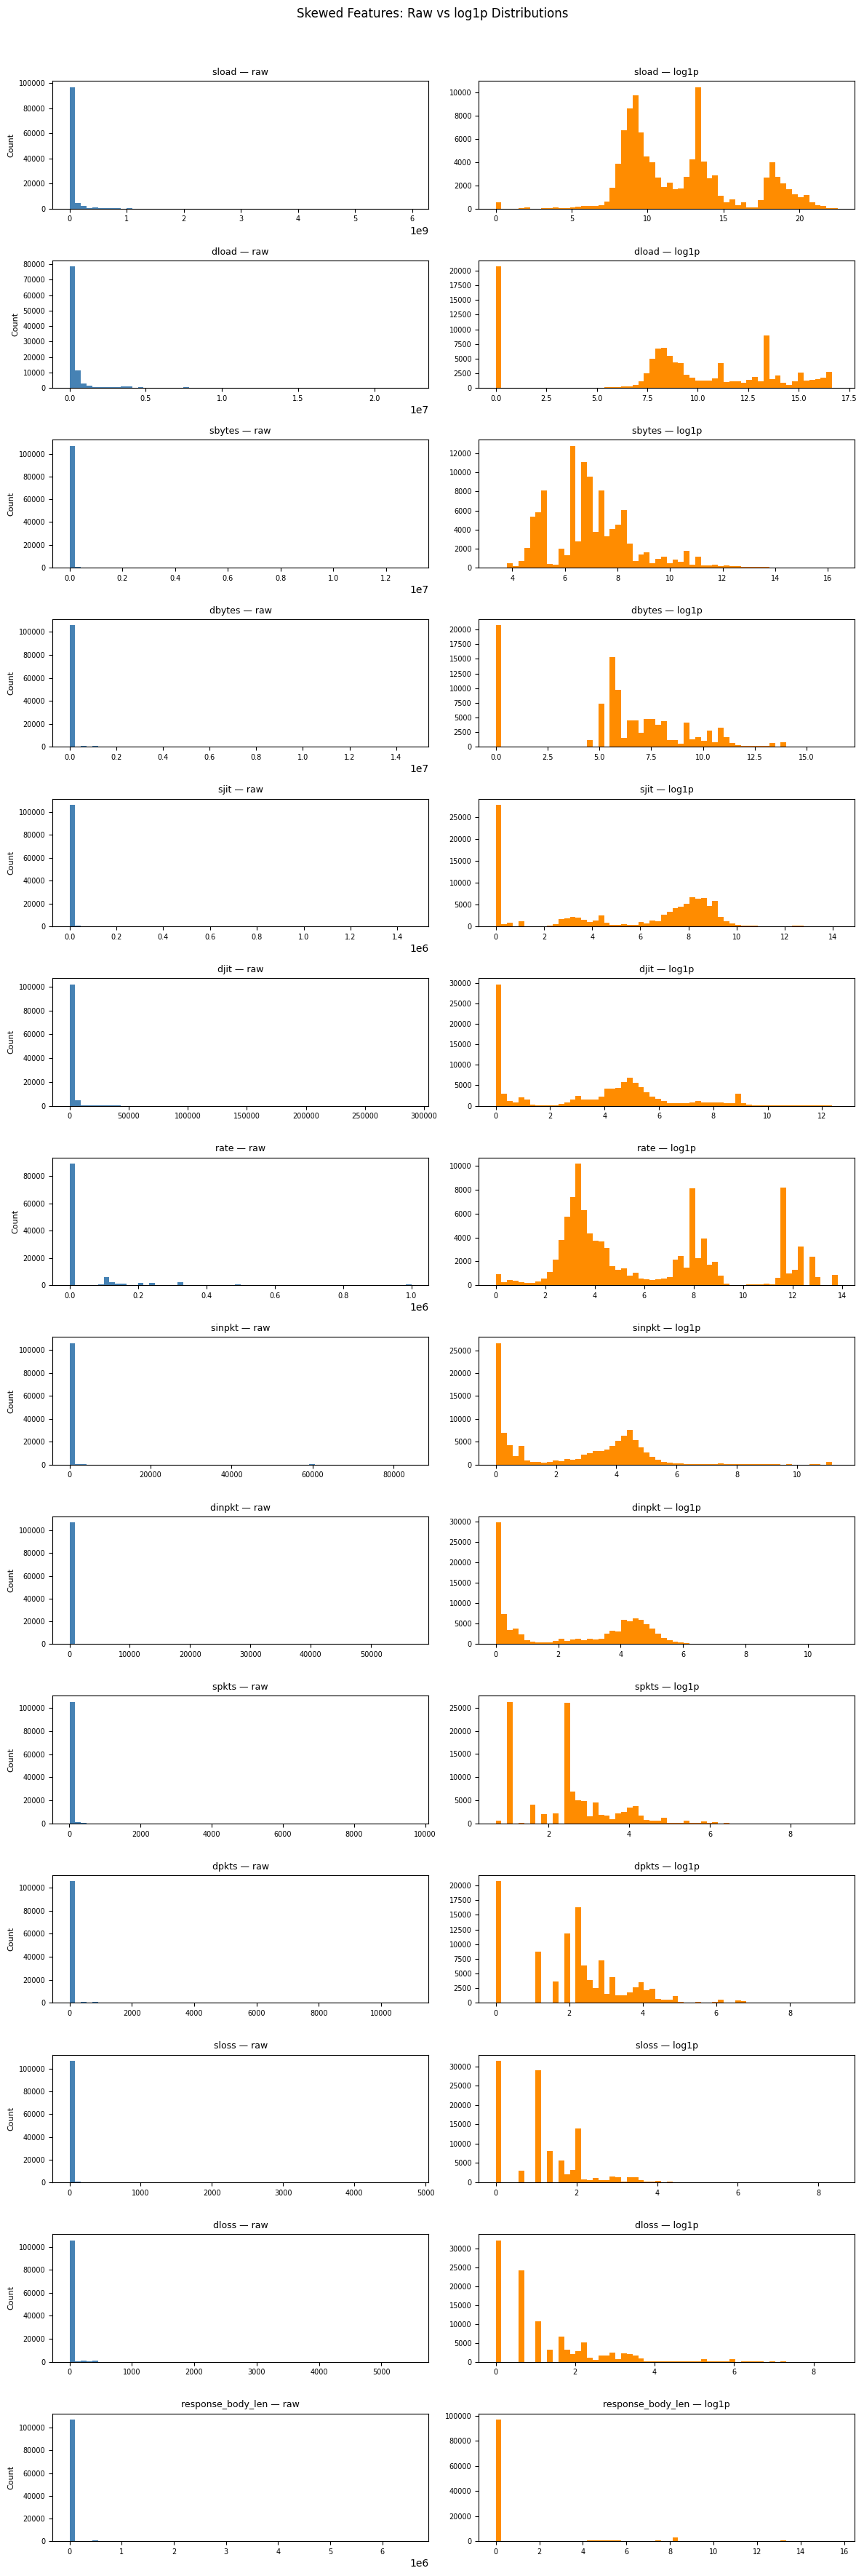
\includegraphics[width=\linewidth,height=0.3\textheight,keepaspectratio]{../report/plots/skewness_plots.png}
    \caption{Raw versus $\log(1+x)$ distributions for the heavily skewed numerical features identified during exploratory analysis.}
    \label{fig:skewness-log1p}
\end{figure}

The categorical exploration in Figure~\ref{fig:categorical-buckets} shows that only a small number of protocol, service, and state values appear frequently. In the raw data, \texttt{proto} has 131 distinct values, but only six of them occur often enough to be informative at scale. The same concentration pattern appears in \texttt{service} and \texttt{state}. This justified collapsing rare categories into an \texttt{other} bucket before one-hot encoding so that the linear and neural models would not be forced to learn from dozens of nearly empty indicator columns.

\begin{figure}[htbp]
    \centering
    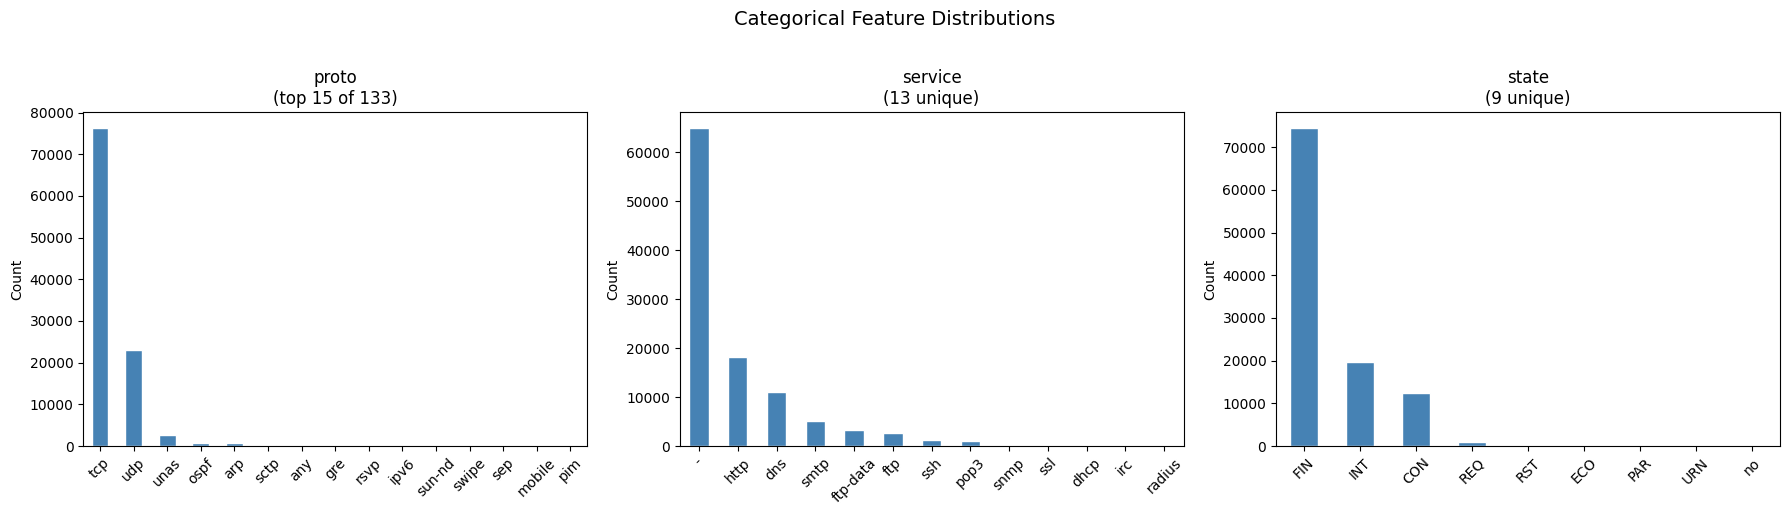
\includegraphics[width=\linewidth,height=0.26\textheight,keepaspectratio]{../report/plots/categorical_plots.png}
    \caption{Frequency distributions of the bucketed categorical features used in the final preprocessing pipeline.}
    \label{fig:categorical-buckets}
\end{figure}

Finally, we examined the numerical correlation structure. The correlation heatmap in Figure~\ref{fig:correlation-heatmap} reveals several highly correlated pairs, especially among throughput- and packet-volume-related variables. We kept these features rather than dropping them aggressively because the tree-based models are robust to correlated inputs and the Logistic Regression baseline can still benefit from keeping distinct but related traffic statistics when regularization is used.

\begin{figure}[htbp]
    \centering
    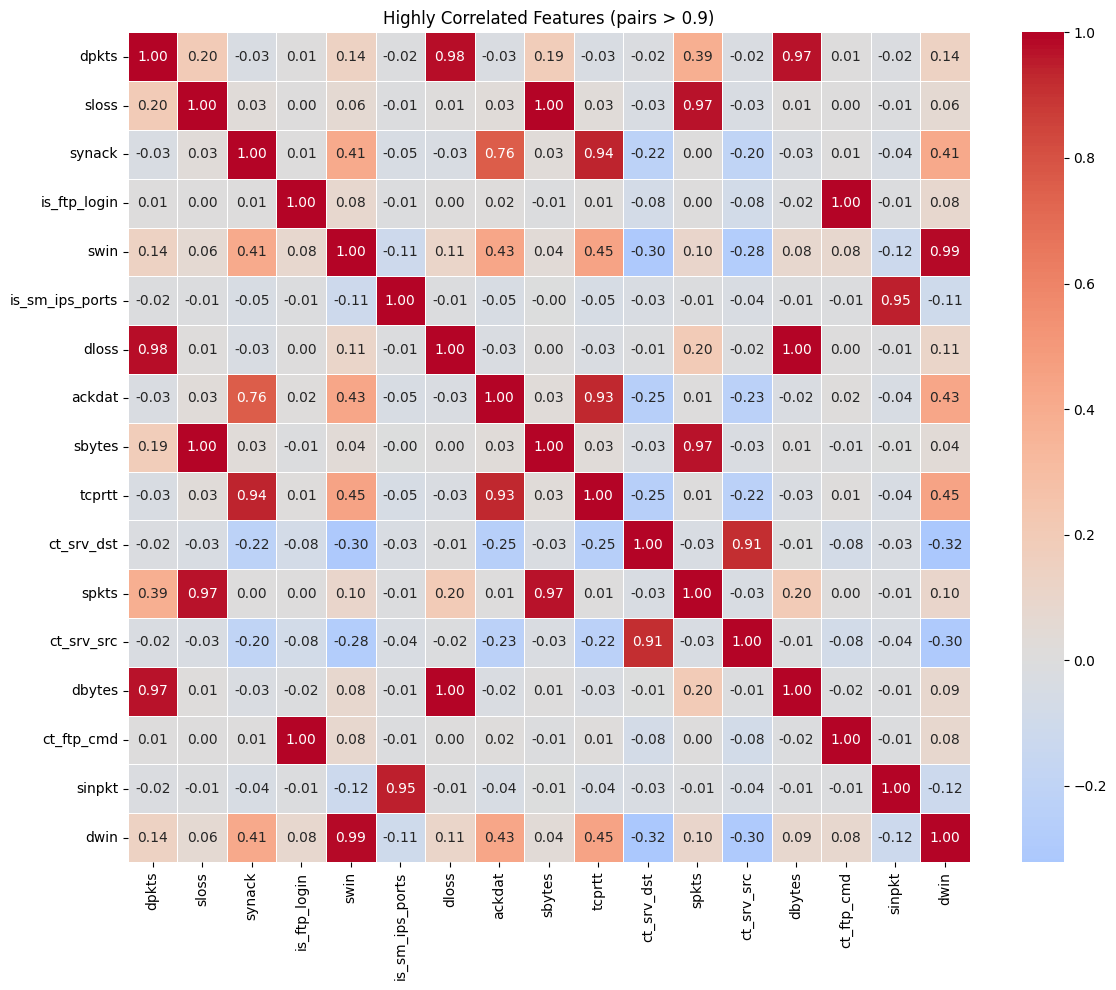
\includegraphics[width=\linewidth,height=0.3\textheight,keepaspectratio]{../report/plots/correlation-heatmap.png}
    \caption{Correlation heatmap over the numerical features used during exploratory analysis.}
    \label{fig:correlation-heatmap}
\end{figure}

\section{Data Cleaning}
The preprocessing code begins by verifying that the dataset contains no missing values; the training split passes this check without requiring imputation. We then remove duplicate rows using all columns except \texttt{id}. This step is important because repeated flows would otherwise inflate downstream metrics and make the held-out evaluation less trustworthy.

We also remove four columns before model fitting:
\begin{itemize}
    \item \texttt{id}, because it is only a row identifier and carries no predictive signal;
    \item \texttt{attack\_cat}, because our task is binary intrusion detection rather than multi-class attack-type prediction;
    \item \texttt{stcpb} and \texttt{dtcpb}, because these TCP base sequence numbers behave like connection-specific identifiers rather than stable behavioural features.
\end{itemize}

\section{Feature Engineering}
The final feature engineering pipeline has three main stages. First, the categorical variables are bucketed by frequency and then one-hot encoded. For \texttt{proto}, we retain \texttt{tcp}, \texttt{udp}, \texttt{unas}, \texttt{arp}, \texttt{ospf}, and \texttt{sctp}. For \texttt{service}, we retain \texttt{-}, \texttt{http}, \texttt{dns}, \texttt{smtp}, \texttt{ftp-data}, \texttt{ftp}, \texttt{ssh}, and \texttt{pop3}. For \texttt{state}, we retain \texttt{FIN}, \texttt{INT}, \texttt{CON}, and \texttt{REQ}. All remaining values are mapped to \texttt{other}. This produces 21 binary indicator columns in total and keeps the categorical representation compact enough for Logistic Regression and the MLP.

Second, we apply $\log(1+x)$ to 14 heavily skewed numerical variables, including load, byte-count, jitter, packet-count, and loss features together with \texttt{response\_body\_len}. We use $\log(1+x)$ instead of $\log(x)$ because many flows have zero values and the shifted transform remains well-defined at zero.

Third, for models that are sensitive to feature scale, we standardize the numerical variables using \texttt{StandardScaler}. The scaler is fit only on the training split and then reused to transform the held-out test split, preventing leakage from the test distribution into the fitted means and variances. The same leakage-avoidance rule is used for categorical encoding: the one-hot column set is learned on the training split and then reindexed on the test split so that unseen or missing categories are handled consistently.

\section{Data Representation and Splits}
We maintain two model-specific representations derived from the same cleaned data:
\begin{itemize}
    \item \textbf{Scaled matrix (\texttt{df\_model})}: 21 one-hot encoded categorical indicators, 14 log-transformed and scaled skewed numerical features, and 23 additional scaled numerical features. This representation is used by Logistic Regression and the Multi-Layer Perceptron.
    \item \textbf{Tree matrix (\texttt{df\_model\_tree})}: the same 21 one-hot encoded indicators combined with the 37 raw numerical features, without standardization. This representation is used by Random Forest and XGBoost, which are largely invariant to monotone rescaling.
\end{itemize}

Both matrices therefore contain 58 predictors plus the label column. To keep preprocessing consistent between training and evaluation, the fitted scaler, one-hot column definitions, and column lists are serialized and reused when transforming the held-out split.

For hyperparameter tuning, we do not carve out a separate validation set from the saved training matrix. Instead, each model uses \texttt{RandomizedSearchCV} with 3-fold cross-validation on the training split, scored by ROC-AUC. Concretely, the 55{,}945-row training matrix is partitioned into three folds for each sampled hyperparameter configuration, while the 107{,}740-row test matrix remains untouched until the final model evaluation. This setup lets us tune models efficiently while preserving a completely held-out dataset for the final comparison study.

\end{spacing}
\newpage
